\section{Introduction}

Recent years have witnessed widespread use of sophistication frameworks such as Hadoop\cite{hadoop}, Spark\cite{spark} and Tez\cite{spark}.
Tremendous effeots have been paid to improve the speed and of large-scale dataparallel systems computing process, from the the low level storage system to scheduling algorithms.

Although highly optimized, DAG computing framworks are derived from MapReduce\cite{mapreduce}, contains a hard barrier between computing stages. The terminology of this barrier is Shuffle. Shuffle contains two parts on the connecting stages. On the side of ancestor stage, shuffle is resoponsible for writing intermediate result to disk. On the side of successor stage, shuffle fetches intermediate result from remote disks in cluster. This shuffle process introduces frequent I/O operations, which result in a significiant performance and cluster utilization decline. For instance, a MapReduce trace analysis from Facebook shows that shuffle accounts for 33\% JCT on average, up to 70\% in shuffle-heavy jobs\cite{manage}.

The straight forward way is to start reduce tasks earlier. Apache Hadoop\cite{hadoop} provides a mechanism, which schedules reduce tasks when a certain portion of map tasks completed. So that the shuffle delay can be mitigated by overlapping execution of reduce phase and map phase. Other publications also purpose solutions to pre-schedule reduce tasks\cite{ihadoop, ishuffle, dynmr}. However this early scheduling of reduce tasks occupies new task slots, which degrades system performance. To this end, we proposed a quetion, \textit{can we efficiently remove shuffle latency without consuming additional task slots?} 
In this paper, we introduce SCache, an auxiliary system to decouple shuffle from computing, pre-schedule tasks and pre-fetch shuffle data for DAG computing frameworks. The workflow of DAG computing with SCache is presented in Figure \ref{fig:workflow}.

\begin{figure}
	\centering
	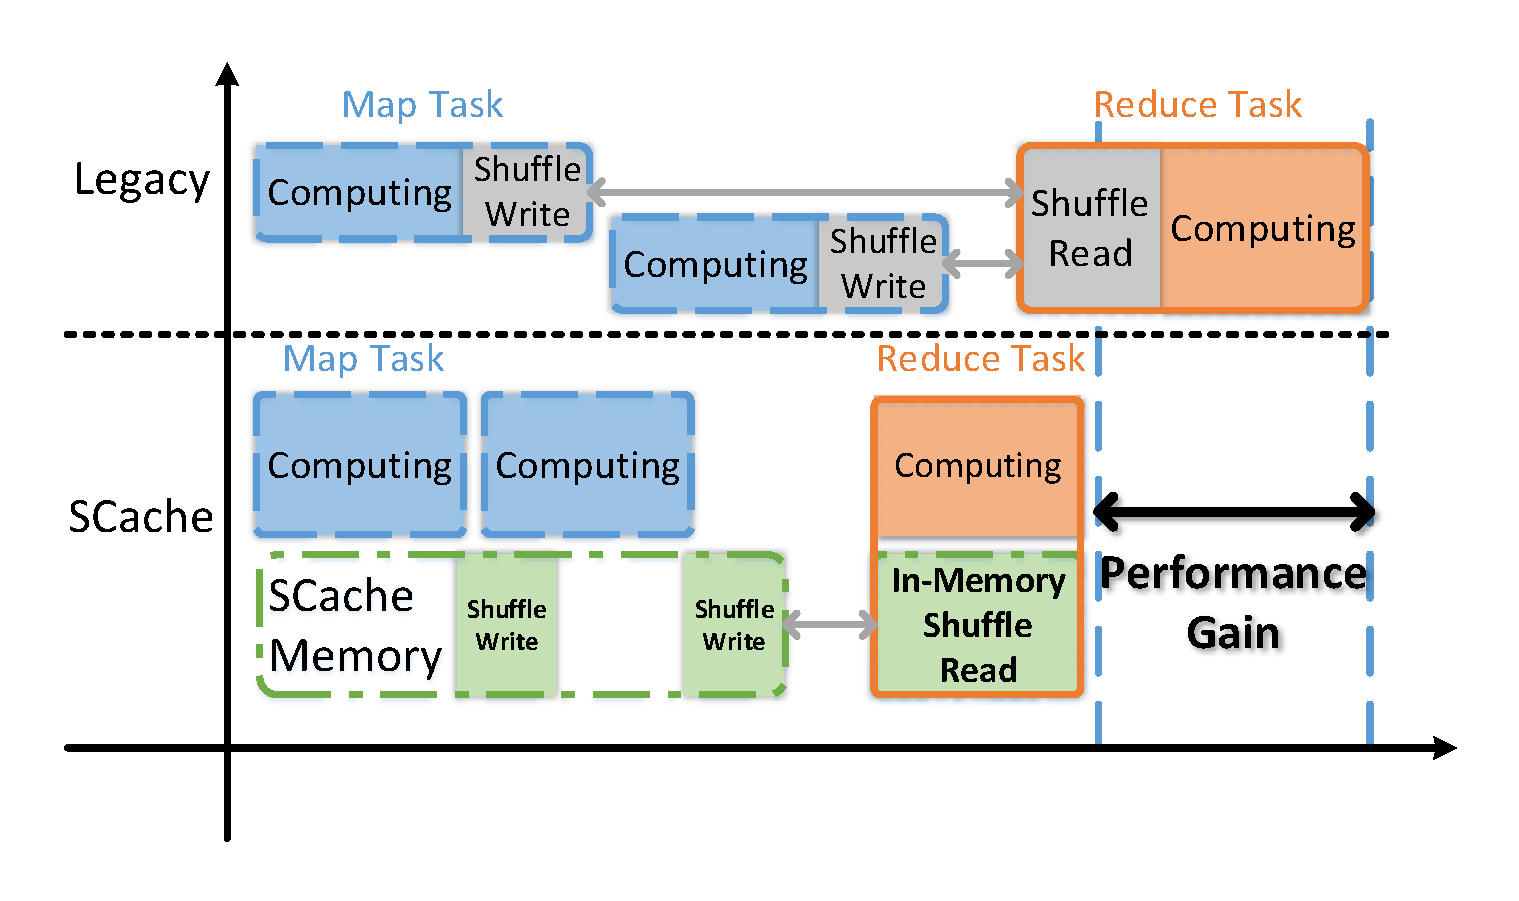
\includegraphics[width=\linewidth]{fig/workflow}
	\caption{Workflow Comparison between Legacy DAG Computing Frameworks and Frameworks with SCache}
	\label{fig:workflow}
\end{figure}
